\documentclass[12pt]{article}	% the type of document is article and font size is 12

% PACKAGES
\usepackage[a4paper, margin=2.5cm]{geometry}
\usepackage{fontspec} 		% package to set font type
\usepackage{anyfontsize}	% custom font sizes
\usepackage{multicol} 		% package to set two column
\usepackage{setspace}		% For controlling line spacing
\usepackage{titlesec}		% advanced title formatting
\usepackage{amsmath} 		% maths formulae
\usepackage{tikz}			% for drawing
\usepackage{graphicx}		% For including images
\usepackage{caption}		% for adding captions
\usepackage{listings}		% for including code
\usepackage{xcolor}			% for coloring code.
\usepackage{booktabs} 		% For professional tables
\usepackage{float}			% For precise positioning
\usepackage[normalem]{ulem} % Enables underlining
\usepackage{xcolor}			% custom colors
\usepackage[backend=biber, style=authoryear]{biblatex}
\usepackage{tikz}			% custom images
\addbibresource{../references.bib} % Path to your .bib file
\usepackage{needspace}
\usepackage{lipsum} 		% For dummy text.
% END PACKAGES

% SETTINGS
\raggedbottom
\setmainfont{Times New Roman}

% END SETTINGS

% BEGIN OUR DOCUMENT.
\begin{document}
	
	% title
	\begin{center}
		{\fontsize{14}{20}\selectfont The Physics of Super Heroes} \\
		\textit{Samson Rapando} \\
	\end{center}
	
	% abstract
	\noindent{\fontsize{11}{11}\selectfont \textbf{Abstract:} \lipsum[1][1-10].  \\
		
	\singlespacing
	
	% begin content
	\begin{multicols}{2}
		
		\section{Introduction}
		
		\lipsum[2][1-3] \parencite{walker2007fundamentals} % from the lipsum text, use paragraph 2, lines 1 to 3
		
		
		\begin{center}
			
\includegraphics[width=0.6\columnwidth]{../images/superhero.png}
			\captionof{figure}{A superhero in costume}
			\label{fig:superhero}
		\end{center}
		
		\noindent As shown in Figure \ref{fig:superhero}, some superheroes have costumes and appear strong visually.
		\noindent \lipsum[1][1-5] \\
		
		\noindent \lipsum[4][1-4] \parencite{kakalios2002physics}
		
		\section{Spider-Man's }
		\lipsum[3][4-9] \\
		
		\noindent \lipsum[2][1-6] \parencite{kakalios2005superheroes} \\
		
		\subsection{Spider-Man's Swinging}
		
		\noindent As shown in Equation \ref{eq:spiderman-equation}, we can see how he swings
		
		\begin{equation}
			T = 2\pi \sqrt{\frac{L}{g}}
			\label{eq:spiderman-equation}
		\end{equation}
		
		\noindent Where
		
		\begin{itemize}
			\item $T$ is the swing period,
			\item $L$ is the length of the web,
			\item $g$ is the gravitational acceleration ($9.81 \, m/s^2$ ).
		\end{itemize}
		
		\noindent Spiderman also experiences a tension calculated as shown in Equation \ref{eq:spiderman-equation-2} \parencite{newton1687principia}
		
		\begin{equation}
			F_T = mg + \frac{mv^2}{r}
			\label{eq:spiderman-equation-2}
		\end{equation}
		
		\noindent \lipsum[2][1-8] \parencite{marvel2021spiderman} \\
		
	
		\subsection{Comparison of Spider-Man to other Superheroes}
		
		\lipsum[1][2-10] \\
		
		\begin{center}
			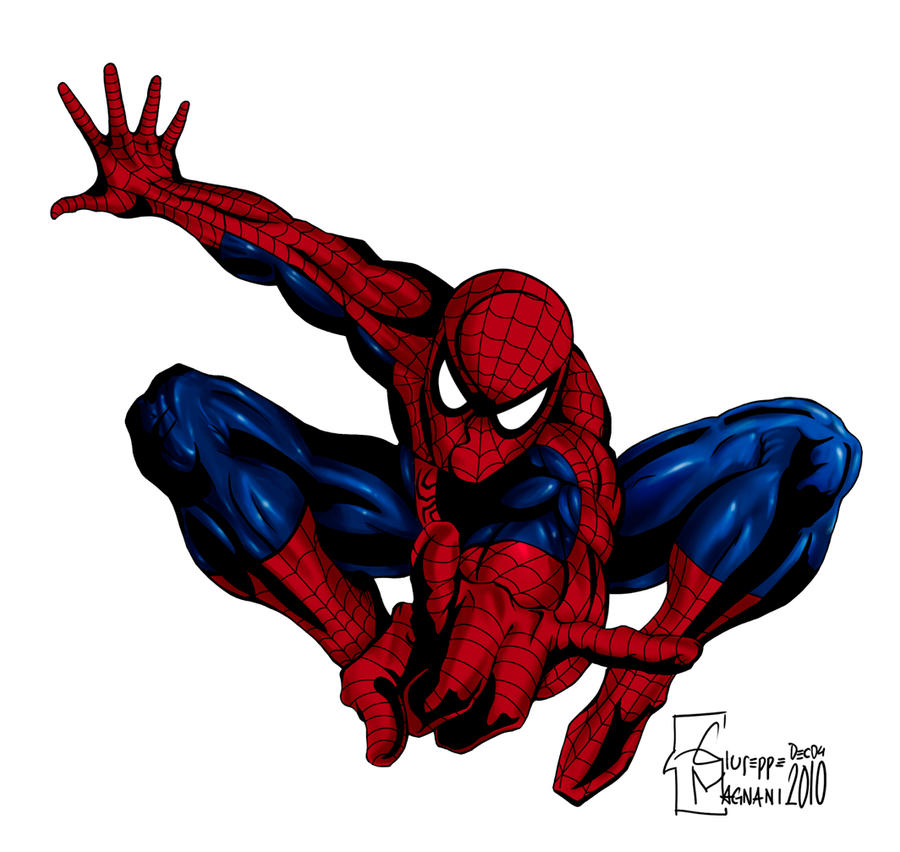
\includegraphics[width=0.6\columnwidth]{../images/spiderman.jpg}
			\captionof{figure}{Spiderman Swinging}
			\label{fig:spiderman-swinging}
		\end{center}
		
		\noindent \lipsum[1][3-9] \\
		
		\begin{center}
			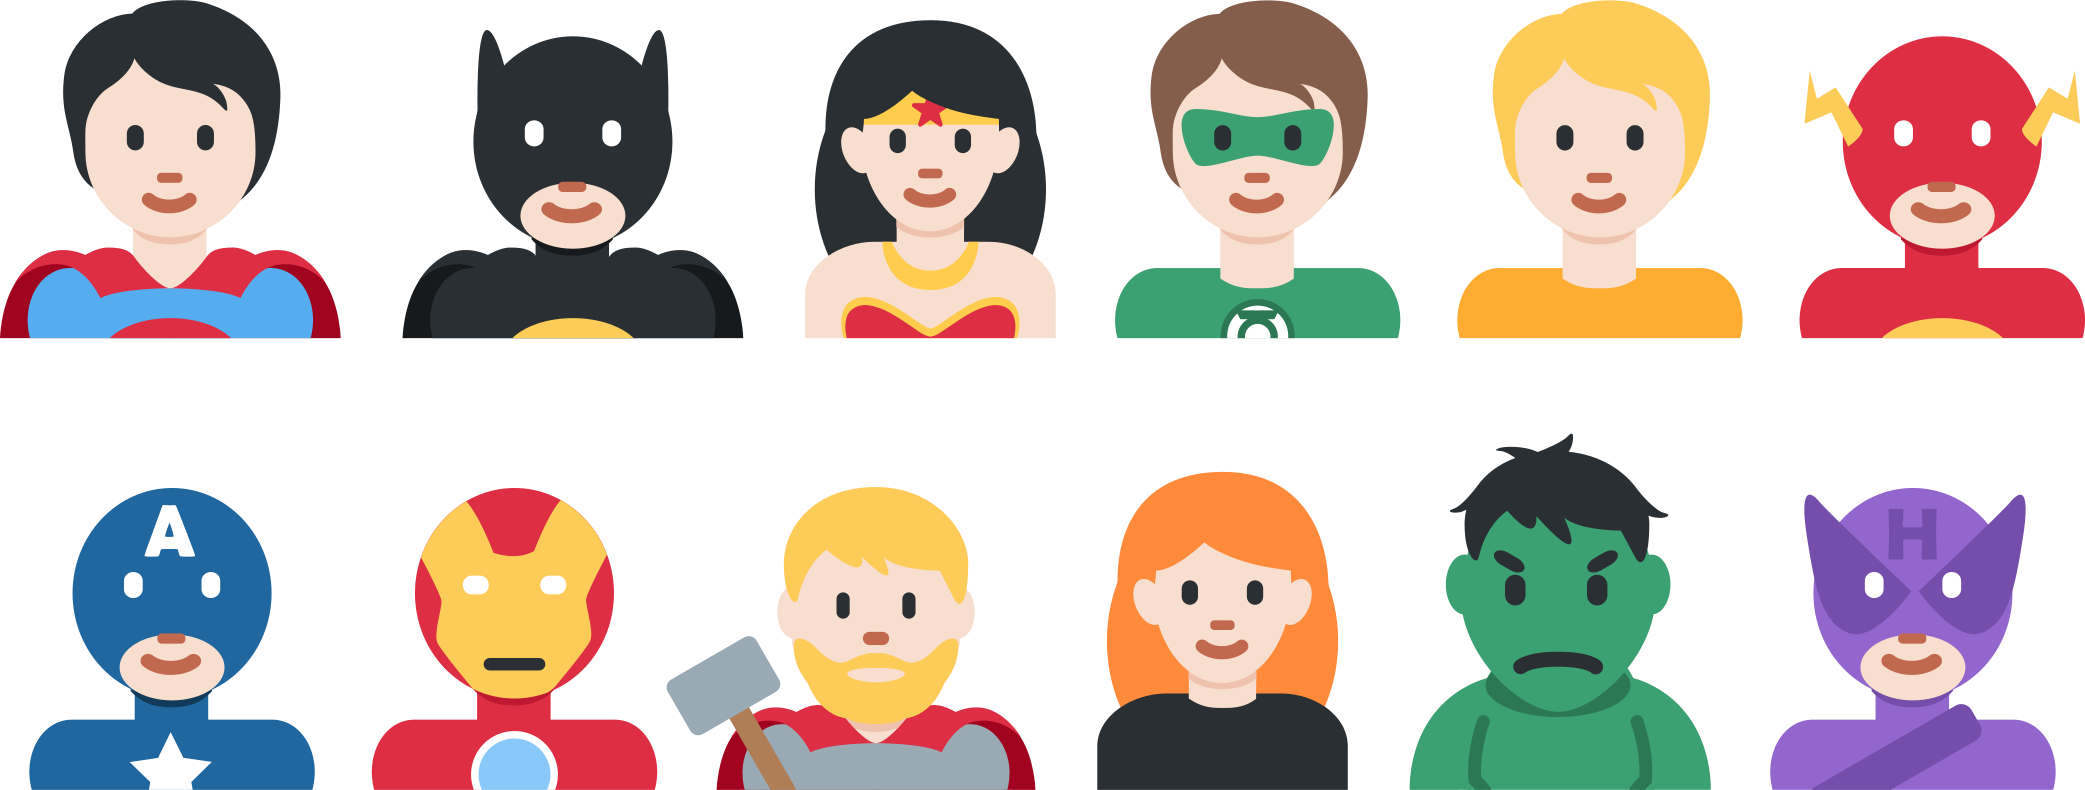
\includegraphics[width=0.6\columnwidth]{../images/Famous_superheroes.png}
			\captionof{figure}{Superheores}
			\label{fig:superheroes}
		\end{center}
		
		\noindent \lipsum[4][1-7] \\
		
		\begin{table}[H]
			\scriptsize
			\centering
			\begin{tabular}{lllc}
				\toprule
				 \textbf{Superhero} & \textbf{Ability} & \textbf{Real World Equivalent} & \textbf{Feasible} \\
				\midrule
				Superman & Flight & Jet Propulsion & No \\
				Spider-Man & Swinging & Pendulum Motion & Yes \\
				The Flash & Speed & Relativity Effects & No \\
				\bottomrule
			\end{tabular}
			\caption{Comparison of Superheroes}
			\label{tab:f1-score}
		\end{table}
		
		\noindent \lipsum[6][1-5] \parencite{dc2021flash}
		
	\end{multicols}
	
	\begin{center}
		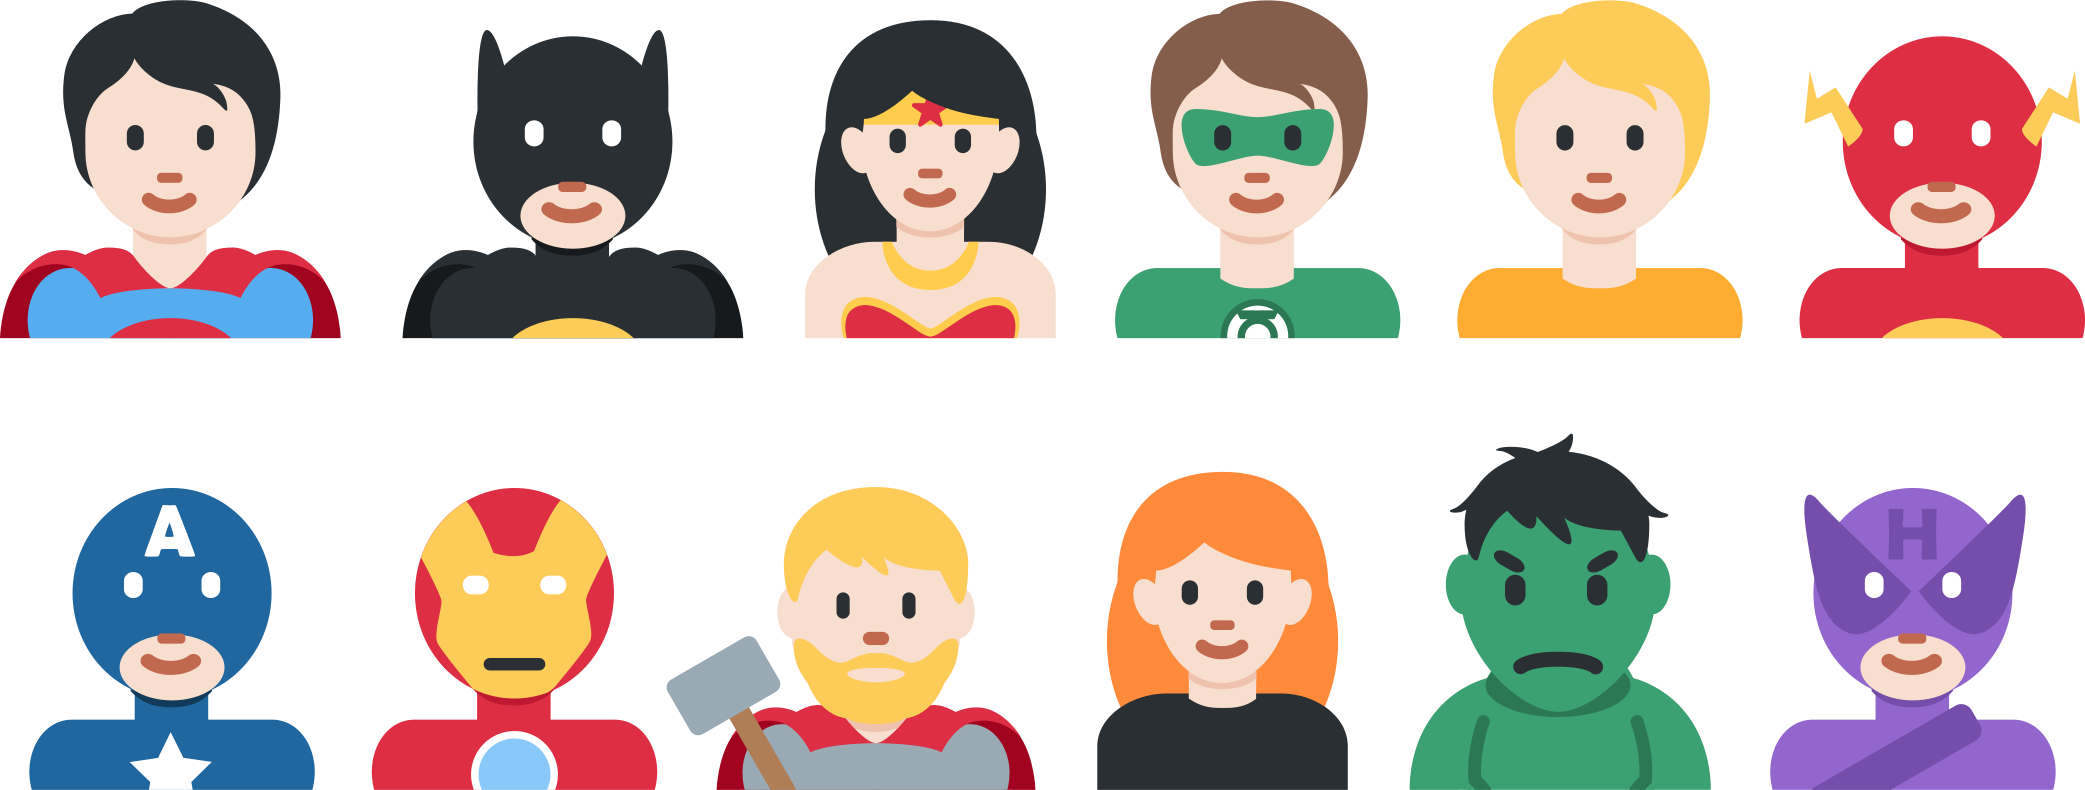
\includegraphics[width=0.6\columnwidth]{../images/Famous_superheroes.png}
		\captionof{figure}{Superheores}
		\label{fig:superheroes2}
	\end{center}
	
	\begin{multicols}{2}
	\noindent \lipsum[1][1-10] \\
	\noindent \lipsum[1][1-10] \\
	\end{multicols}
	
	
	\printbibliography

	
\end{document}